\begin{exercise}
Wenden Sie verschiedene lineare Mehrschrittverfahren auf das Anfangswertproblem zur\\
Wärmeleitungsgleichung aus Aufgabe 29 an. Verwenden Sie dazu:
\begin{enumerate}[label = \textbf{\alph*)}]
  \item Das Adams-Bashforth-Verfahren mit $k = 3$.
  \item Die Adams-Moulton-Verfahren mit $k = 2,3$.
  \item Das BDF-Verfahren
  \begin{align*}
    y_{\ell + 1} - \frac{48}{25}y_{\ell} + \frac{36}{25}y_{\ell - 1} - \frac{16}{25}y_{\ell - 2}
    + \frac{3}{25}y_{\ell - 3} = h\frac{12}{25}f(t_{\ell + 1},y_{\ell + 1}).
  \end{align*}
\end{enumerate}
Optimieren Sie jeweils die Schrittweite $h$, also wählen Sie $h$ so groß wie möglich,
wobei $\|U(t)\|_{\infty}$ aber noch in der Zeit fallen sollte. Was beobachten Sie? \\
\textit{Hinweis:} Für die impliziten Verfahren benötigen Sie keine Newton-Iteration,
sondern können die auftretenden Gleichungen explizit lösen. Beachten Sie dabei Aufgabe 29c.
\end{exercise}
\begin{solution}
\begin{align}
  M_h := \frac{1}{h^2}\begin{pmatrix}
    -2 & 1 & &  \\
    1 & -2 & \ddots & \\
    & \ddots & \ddots & 1 \\
    & & 1 & -2
  \end{pmatrix}
  \in \R^{(N-1)\times (N-1)}
\end{align}
\begin{align}\label{awp}
  U_h^{\prime} = M_hU_h, \qquad U_h(0) = G
\end{align}
Berechnen Sie die Lösung des Anfangswertproblems \eqref{awp} auf dem Intervall
$[0,1]$ numerisch. Der Anfangswert $G$ soll die Funktion
$g(x) := \exp\left(-30\left(x-\frac{1}{2}\right)^2\right)$ nodal approximieren, also
$G_i := g\left(\frac{i}{N}\right)$ für $i = 1,\dots,N-1$.
\begin{figure}
    \centering
    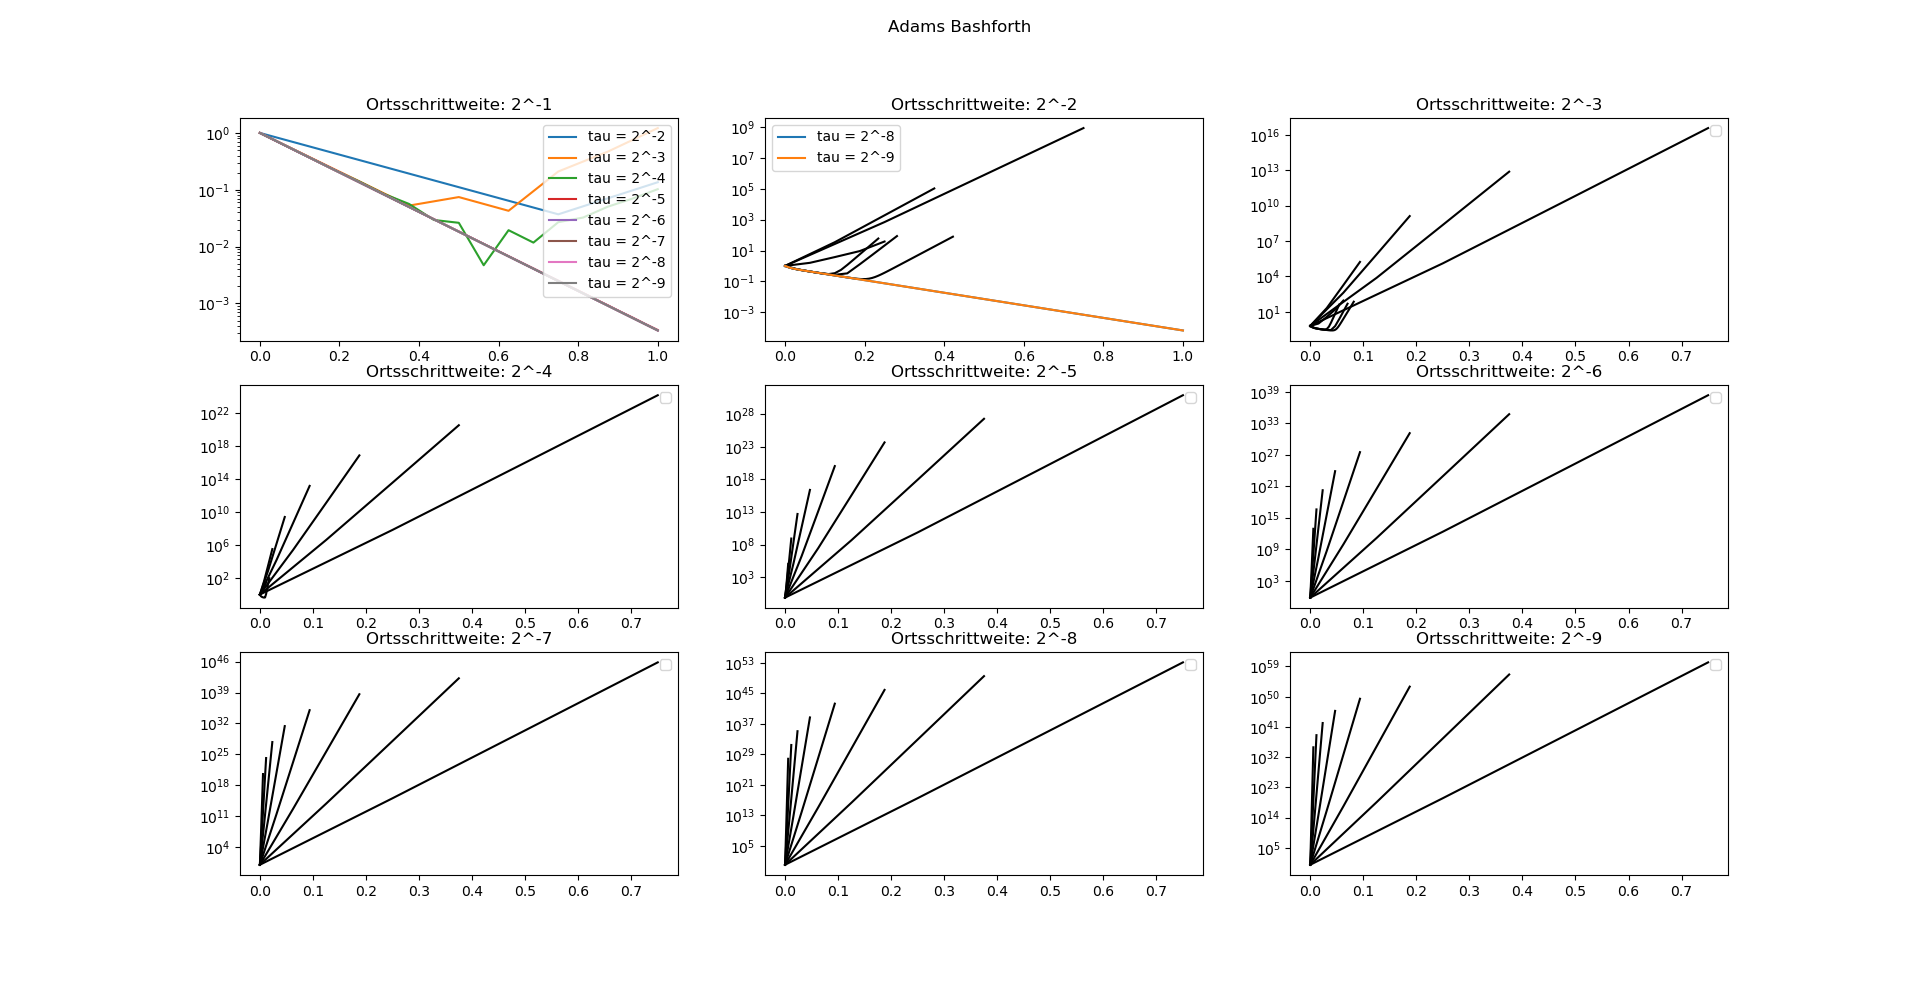
\includegraphics[width=\linewidth]{plot1.png}
\end{figure}
\begin{figure}
    \centering
    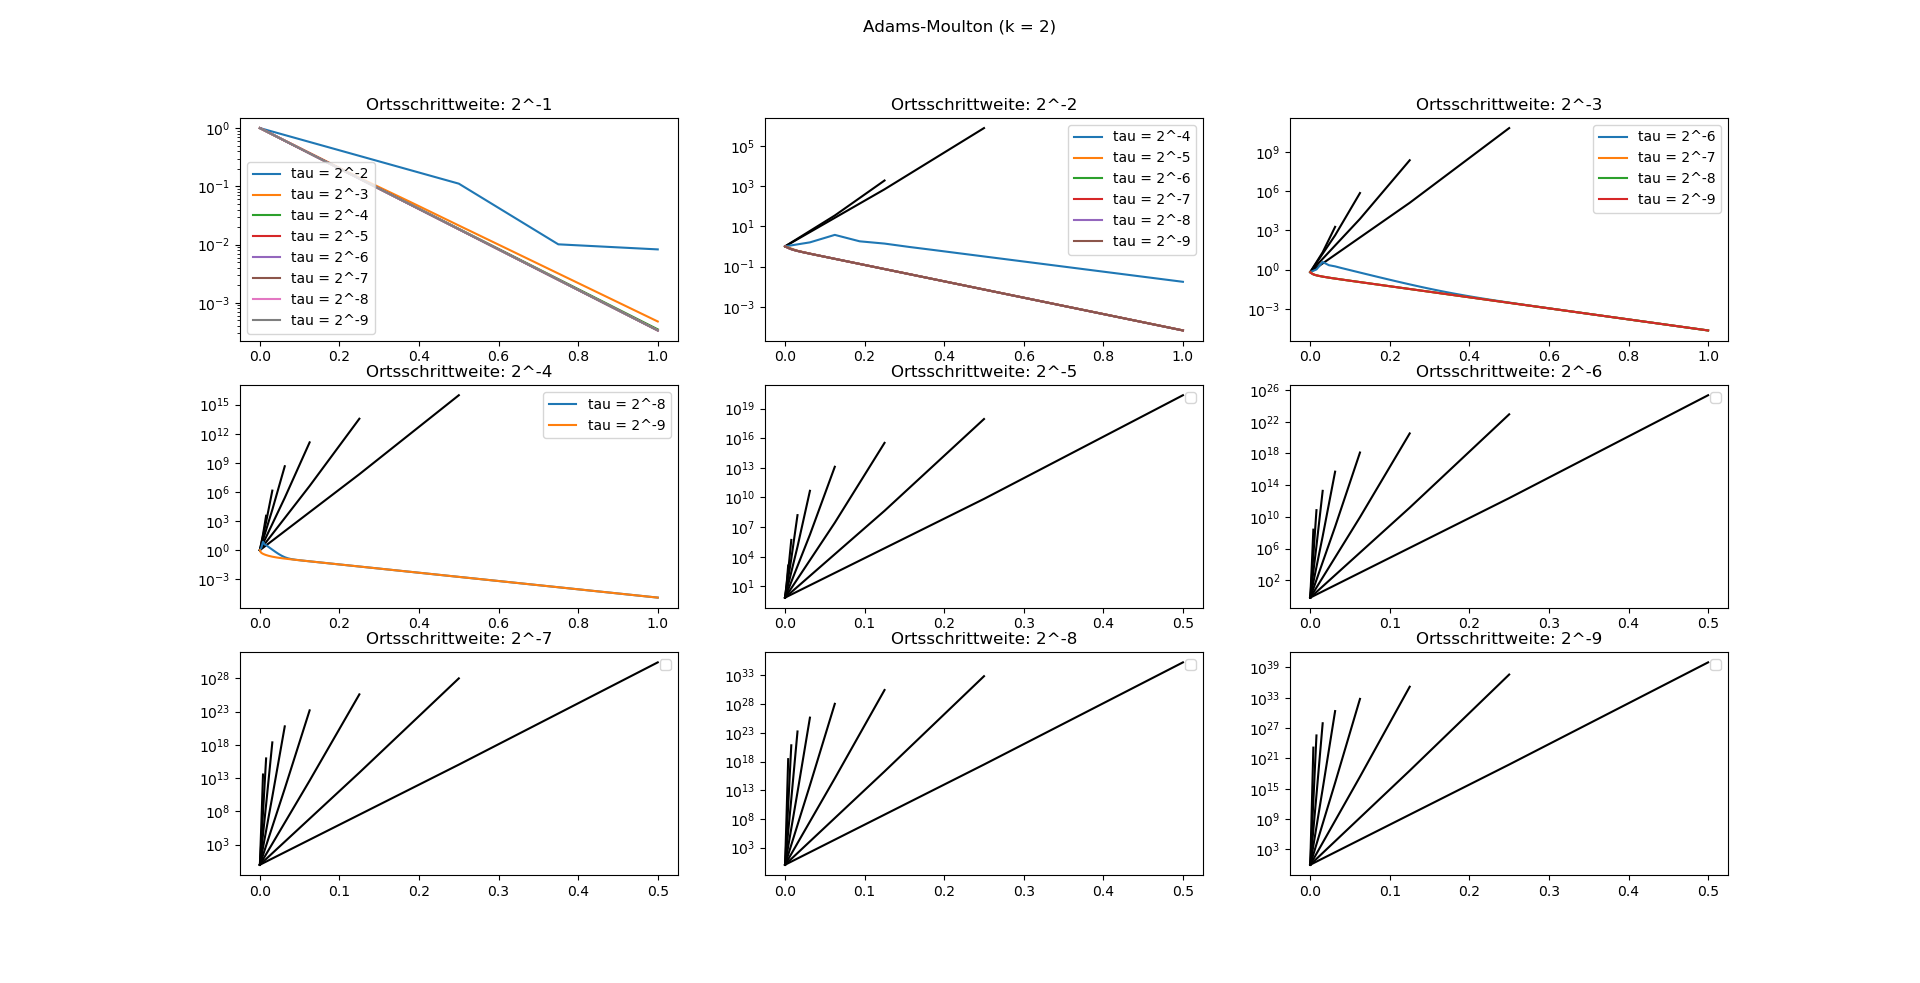
\includegraphics[width=\linewidth]{plot2.png}
\end{figure}
\begin{figure}
    \centering
    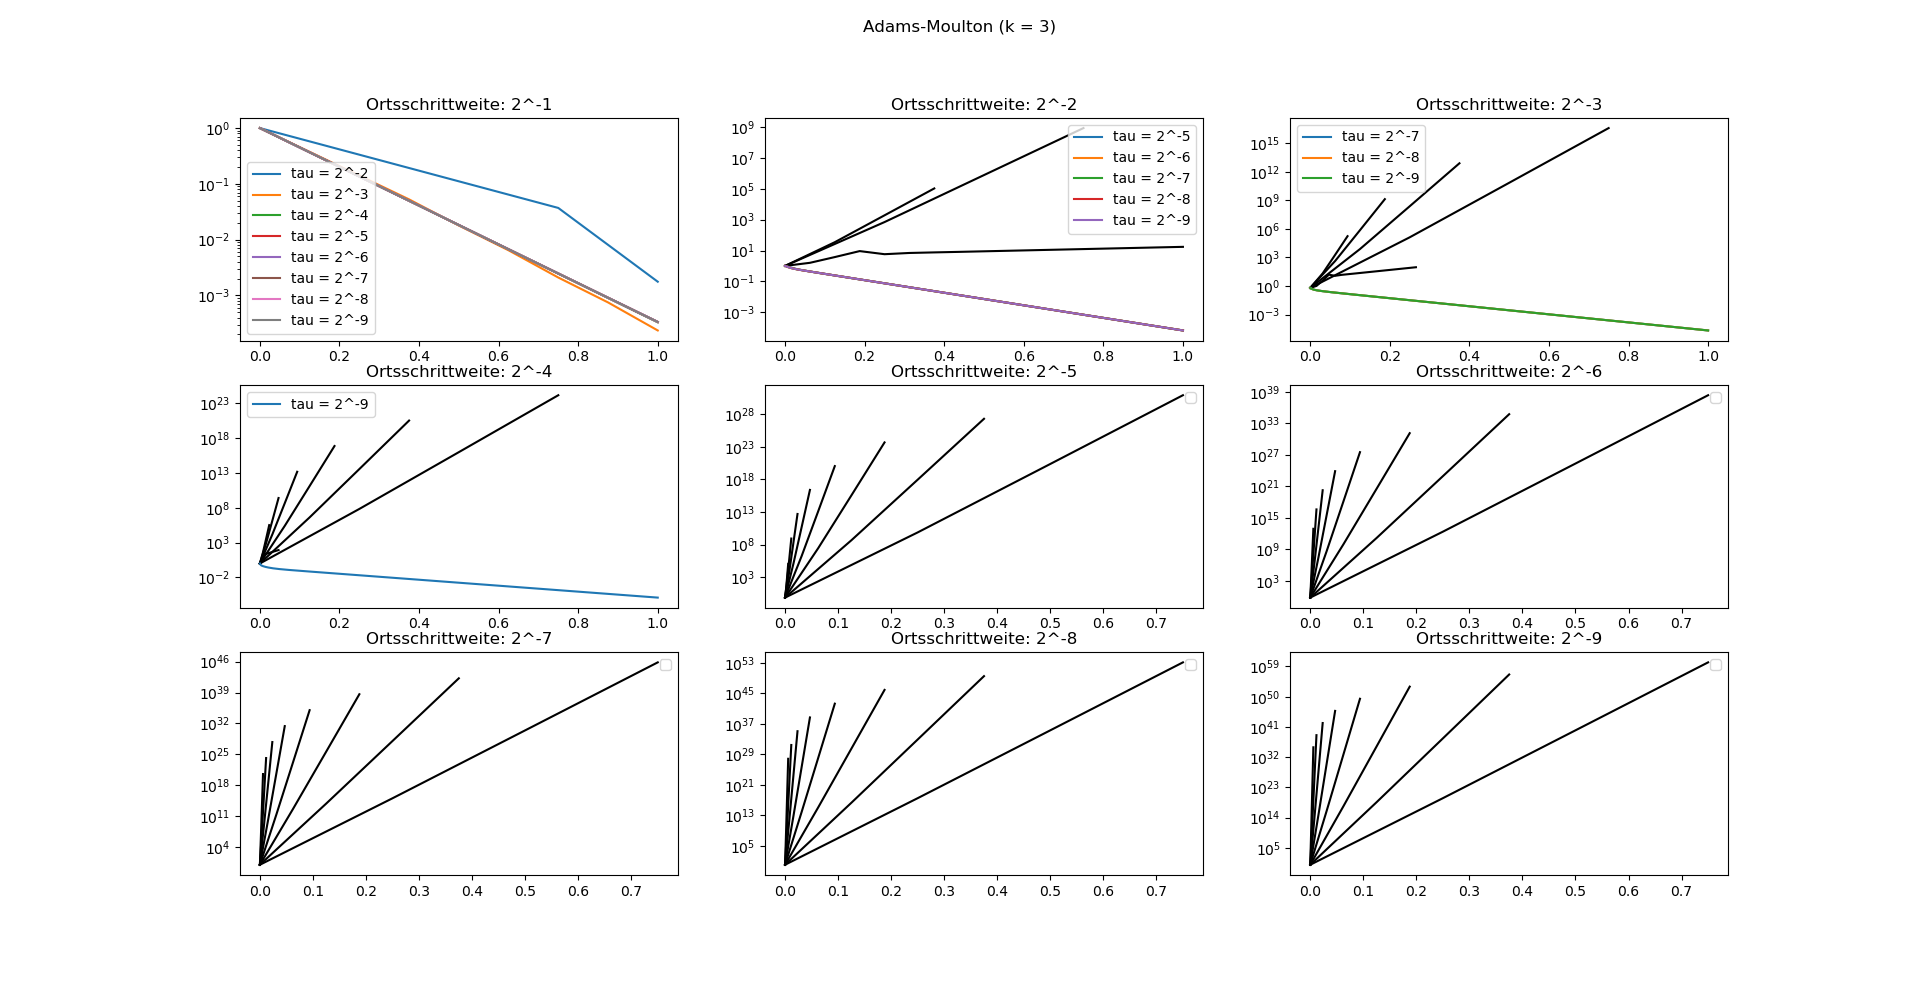
\includegraphics[width=\linewidth]{plot3.png}
\end{figure}
\begin{figure}
    \centering
    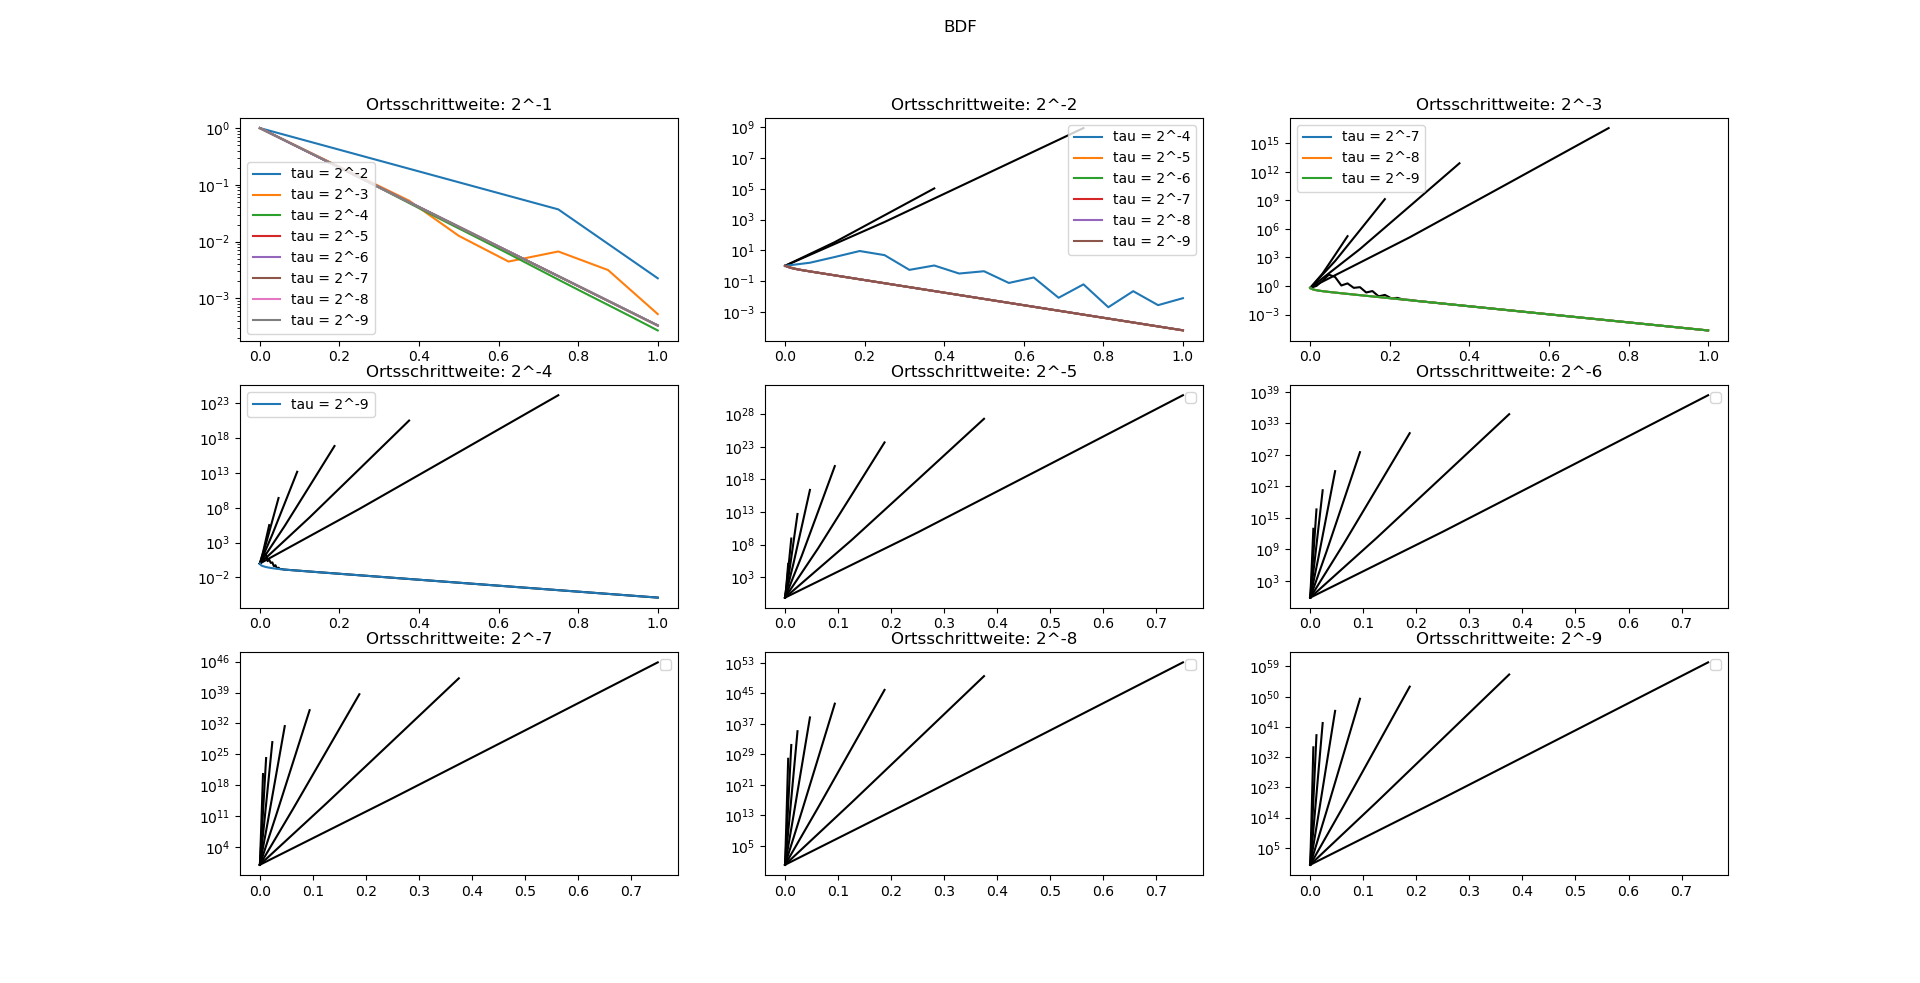
\includegraphics[width=\linewidth]{plot4.png}
\end{figure}
\end{solution}
